\documentclass{beamer}
\newcommand{\beaa}{\begin{eqnarray*}}
\newcommand{\eeaa}{\end{eqnarray*}}
\newcommand{\bea}{\begin{eqnarray}}
\newcommand{\eea}{\end{eqnarray}}
\setbeamercolor{title}{fg=orange!50!black} % instead of above (dark background, white foreground)
\setbeamertemplate{frametitle}[default][center] % by default have it center-justified
%\setbeamercolor{frametitle}{fg=white,bg=orange!50!black}
\setbeamercolor{frametitle}{fg=orange!50!black} % instead of above (dark background, white foreground)
\setbeamercolor{structure}{fg=orange!50!black}
\setbeamertemplate{footline}[frame number]
%\setbeamertemplate{navigation symbols}{} % suppress all navigation symbols
\usepackage[english]{babel}
\usepackage[latin1]{inputenc}
\usepackage{times}
\usepackage[T1]{fontenc}

\title[Spatial Models and Computation] % (optional, use only with long paper titles)
% {Gaussian processes for complex computer models and classification}
%{Computationally Intensive Probability and Statistics}
%\subtitle{(A Short Course)}
{A Short Course on Computationally Intensive Probability and Statistics}
%\subtitle{(A Short Course)}
\author{Murali Haran}

\institute[Penn State] % (optional, but mostly needed)
{
%  \inst{1}%
  Department of Statistics\\
  Penn State University\\
\vspace{0.2in}
%(references Rasmussen and Williams (2006) and others.)
}
%
\date[SOS 03-2006] % (optional, should be abbreviation of conference name)
{University of Split\\ September 2017}
%{Theory of Continuous Space and Space-Time Processes. \\SAMSI, November 2009}

%## Total: around 80 slides since 80x2 = 160 = 2 hr.40mins.

%## 2 slides: intro
%## 10 slides: computer models
%## 20 slides: computer model calibration (including toy + real examples?)
%## 10 slides: GPs for classification
%## 20 slides: Computing: MCMC algorithms, Laplace approximation

% \theoremstyle{remark}
% \newtheorem{example}{Example}
% \usepackage{geometry}
% %\geometry{hmargin=1.025in,vmargin={1.25in,0.75in},nohead,footskip=0.5in}
% \geometry{hmargin=2.5cm,vmargin={2.5cm,2.5cm},nohead,footskip=0.5in}
% \renewcommand{\baselinestretch}{1.21} 
\newcommand{\Real}{{\mathbb R}}
\newcommand{\boldY}{{\bf Y}}
\newcommand{\boldZ}{{\bf Z}}
\newcommand{\boldR}{{\bf R}}
\newcommand{\boldz}{{\bf z}}
\newcommand{\boldC}{{\bf C}}
\newcommand{\boldB}{{\bf B}}
\newcommand{\boldI}{{\bf I}}
\newcommand{\bell}{ \mbox{\boldmath $\ell$}}
\newcommand{\btheta}{ \mbox{\boldmath $\theta$}}
\newcommand{\bphi}{ \mbox{\boldmath $\phi$}}
\newcommand{\bPhi}{ \mbox{\boldmath $\Phi$}}
\newcommand{\bmu}{ \mbox{\boldmath $\mu$}}
\newcommand{\bxi}{ \mbox{\boldmath $\xi$}}
\newcommand{\boldeta}{ \mbox{\boldmath $\eta$}}
\newcommand{\beq}{\begin{equation}}
\newcommand{\eeq}{\end{equation}}
\newcommand{\beqstar}{\begin{equation*}}
\newcommand{\eeqstar}{\end{equation*}}
\newcommand{\bthet}{ \mbox{\boldmath $\theta$}}
\newcommand{\blambda}{ \mbox{\boldmath $\lambda$}}
\newcommand{\bet}{ \mbox{\boldmath $\eta$}}
\newcommand{\bepsilon}{ \mbox{\boldmath $\epsilon$}}
\newcommand{\bdelta}{ \mbox{\boldmath $\delta$}}
\newcommand{\bnu}{ \mbox{\boldmath $\nu$}}
\newcommand{\bPsi}{ \mbox{\boldmath $\Psi$}}
\newcommand{\bY}{ {\bf Y} }
\newcommand{\by}{ {\bf y} }
\newcommand{\bM}{ {\bf M} }
\newcommand{\bU}{ {\bf U} }
\newcommand{\bu}{ {\bf u} }
\newcommand{\br}{ {\bf r} }
\newcommand{\bK}{ {\bf K} }
\newcommand{\bz}{ {\bf z} }
\newcommand{\bd}{ {\bf d} }
\newcommand{\bh}{ {\bf h} }
\newcommand{\bw}{ {\bf w} }
\newcommand{\bs}{ {\bf s} }
\newcommand{\bg}{ {\bf g} }
\newcommand{\bt}{ {\bf t} }
\newcommand{\bv}{ {\bf v} }
\newcommand{\bx}{ {\bf x} }
\newcommand{\bZ}{{\bf Z}}
\newcommand{\bX}{{\bf X}}
\newcommand{\bW}{{\bf W}}
\newcommand{\bE}{{\bf E}}
\newcommand{\bbeta}{ \mbox{\boldmath $\beta$}}
\newcommand{\bmuhat}{ \mbox{\boldmath $\hat{\mu}$}}
\newcommand{\beas}{\begin{eqnarray*}}
\newcommand{\eeas}{\end{eqnarray*}}
\renewcommand{\familydefault}{\sfdefault}
\renewcommand{\baselinestretch}{1.3}
\newcommand{\Nstar}{N^{*}}
\newcommand{\taustar}{\tau^{*}}
\newcommand{\alphatilde}{\tilde{\alpha}}
\newcommand{\lambdaT}{\lambda_{\theta}}
%\newcommand{\xprime}{x^{'}}
%\newcommand{\mprime}{m^{'}}
\newcommand{\bOne}{ {\bf 1} }
\newcommand{\bZero}{ {\bf 0} }
\newcommand{\xprime}{x'}
\newcommand{\nprime}{n'}
\newcommand{\mprime}{m'}
\newcommand{\bTheta}{ \mbox{\boldmath $\Theta$}}

\newcommand{\Cset}{\cal C}
\newcommand{\taueps}{\tau_{\epsilon}}
\newcommand{\Galpha}{G_{\alpha}}
\newcommand{\boldzpr}{{\bf z^{'}}}
\newcommand{\alphapr}{\alpha^{'}}
\newcommand{\tauepspr}{\taueps^{'}}
\newcommand{\Nkappa}{N_{\kappa}}
\def\baro{\vskip  .2truecm\hfill \hrule height.5pt \vskip  .2truecm}
\def\barba{\vskip -.1truecm\hfill \hrule height.5pt \vskip .4truecm}
\newcommand{\Matern}{Mat\'{e}rn }
\newcommand{\Rcode}{{\color{green} {R command: }}}
\newcommand{\bigoh}{\mathcal{O}}
\newcommand{\figtwobytwo}[4]
{
\begin{tabular}{cc}
    {{\resizebox*{0.47\textwidth}{0.35\textheight}
        {\rotatebox{0}{\includegraphics{#1}}}} \par}&
    {{\resizebox*{0.47\textwidth}{0.35\textheight}
        {\rotatebox{0}{\includegraphics{#2}}}} \par}\\
    {{\resizebox*{0.47\textwidth}{0.35\textheight}
        {\rotatebox{0}{\includegraphics{#3}}}} \par}&
    {{\resizebox*{0.47\textwidth}{0.35\textheight}
        {\rotatebox{0}{\includegraphics{#4}}}} \par}\\
\end{tabular}
}
\newcommand{\figtwobytwoA}[4]
{
\begin{tabular}{cc}
    {{\resizebox*{0.35\textwidth}{0.3\textheight}
        {\rotatebox{0}{\includegraphics{#1}}}} \par}&
    {{\resizebox*{0.35\textwidth}{0.3\textheight}
        {\rotatebox{0}{\includegraphics{#2}}}} \par}\\
    {{\resizebox*{0.35\textwidth}{0.3\textheight}
        {\rotatebox{0}{\includegraphics{#3}}}} \par}&
    {{\resizebox*{0.35\textwidth}{0.3\textheight}
        {\rotatebox{0}{\includegraphics{#4}}}} \par}\\
\end{tabular}
}
\newcommand{\figtwo}[2]
{
\begin{tabular}{cc}
    {{\resizebox*{0.35\textwidth}{0.2\textheight}
        {\rotatebox{0}{\includegraphics{#1}}}} \par}&
    {{\resizebox*{0.35\textwidth}{0.2\textheight}
        {\rotatebox{0}{\includegraphics{#2}}}} \par}\\
\end{tabular}
}
\newcommand{\figtwoA}[2]
{
\begin{tabular}{cc}
%    {{\resizebox*{0.33\textwidth}{0.24\textheight}
    {{\resizebox*{0.45\textwidth}{0.45\textheight}
        {\rotatebox{0}{\includegraphics{#1}}}} \par}&
    {{\resizebox*{0.45\textwidth}{0.45\textheight}
        {\rotatebox{0}{\includegraphics{#2}}}} \par}\\
\end{tabular}
}
\newcommand{\figtwoB}[2]
{
\begin{tabular}{cc}
%    {{\resizebox*{0.33\textwidth}{0.24\textheight}
    {{\resizebox*{0.6\textwidth}{0.7\textheight}
        {\rotatebox{0}{\includegraphics{#1}}}} \par}&
    {{\resizebox*{0.6\textwidth}{0.7\textheight}
        {\rotatebox{0}{\includegraphics{#2}}}} \par}\\
\end{tabular}
}
\newcommand{\figtwoC}[4]
{
\begin{tabular}{cc}
%    {{\resizebox*{0.33\textwidth}{0.24\textheight}
  #3 & #4 \\
    {{\resizebox*{0.47\textwidth}{0.55\textheight}
        {\rotatebox{0}{\includegraphics{#1}}}} \par}
     &
    {{\resizebox*{0.47\textwidth}{0.55\textheight}
        {\rotatebox{0}{\includegraphics{#2}}}} \par}\\
\end{tabular}
}

%\newcommand{\figone}[1]
%{
%  \begin{center}
%    {{\resizebox*{0.95\textwidth}{0.7\textheight}
%        {\rotatebox{270}{\includegraphics{#1}}}} \par}
%  \end{center}
%  }

\newcommand{\figoneA}[1]
{
  \begin{center}
    {{\resizebox*{0.35\textwidth}{0.35\textheight}
        {\rotatebox{0}{\includegraphics{#1}}}} \par}
  \end{center}
  }

\newcommand{\figoneAA}[1]
{
  \begin{center}
    {{\resizebox*{1\textwidth}{0.3\textheight}
        {\rotatebox{0}{\includegraphics{#1}}}} \par}
  \end{center}
  }

\newcommand{\figoneAAbig}[1] % Sham's version
 {
  \begin{center}
    {{\resizebox*{0.7\textwidth}{0.7\textheight}
        {\rotatebox{0}{\includegraphics{#1}}}} \par}
  \end{center}
  }
  
 
  \newcommand{\figoneAB}[1]
{
  \begin{center}
    {{\resizebox*{0.6\textwidth}{0.6\textheight}
        {\rotatebox{0}{\includegraphics{#1}}}} \par}
  \end{center}
  }
  
    \newcommand{\figoneAC}[1]
{
  \begin{center}
    {{\resizebox*{0.65\textwidth}{0.65\textheight}
        {\rotatebox{0}{\includegraphics{#1}}}} \par}
  \end{center}
  }

    \newcommand{\figoneAD}[1]
{
  \begin{center}
    {{\resizebox*{0.70\textwidth}{0.70\textheight}
        {\rotatebox{0}{\includegraphics{#1}}}} \par}
  \end{center}
  }

\newcommand{\figonebig}[1]
{
  \begin{center}
    {{\resizebox*{0.7\textwidth}{0.7\textheight}
        {\rotatebox{0}{\includegraphics{#1}}}} \par}
  \end{center}
  }
\newcommand{\figtwoAA}[2]
{
\begin{tabular}{cc}
%    {{\resizebox*{0.33\textwidth}{0.24\textheight}
    {{\resizebox*{0.45\textwidth}{0.45\textheight}
        {\rotatebox{0}{\includegraphics{#1}}}} \par}&
    {{\resizebox*{0.45\textwidth}{0.45\textheight}
        {\rotatebox{0}{\includegraphics{#2}}}} \par}\\
\end{tabular}
}

%\newcommand{\figonesmall}[1]
%{
%  \begin{center}
%    {{\resizebox*{0.475\textwidth}{0.35\textheight}
%        {\rotatebox{0}{\includegraphics{#1}}}} \par}
%  \end{center}
%  }

%\newcommand{\figonerotate}[1]
%{
%  \begin{center}
%    {{\resizebox*{0.7\textwidth}{0.7\textheight}
%%    {{\resizebox*{0.95\textwidth}{0.7\textheight}
%        {\rotatebox{0}{\includegraphics{#1}}}} \par}
%  \end{center}
%  }
% \newcommand{\figonerotatemedium}[1]
% {
%  \begin{center}
%    {{\resizebox*{0.95\textwidth}{0.7\textheight}
%    {{\resizebox*{0.855\textwidth}{0.63\textheight}
%    {{\resizebox*{0.665\textwidth}{0.49\textheight} % with image-transform-autocrop in gimp (R map files)
%        {\rotatebox{0}{\includegraphics{#1}}}} \par}
%  \end{center}
%  }
%\newcommand{\figonerotatemediumsmall}[1]
%{
%  \begin{center}
%%    {{\resizebox*{0.95\textwidth}{0.7\textheight}
%%    {{\resizebox*{0.855\textwidth}{0.63\textheight}
%    {{\resizebox*{0.532\textwidth}{0.392\textheight} % with image-transform-autocrop in gimp (R map files)
%        {\rotatebox{0}{\includegraphics{#1}}}} \par}
%  \end{center}
%  }
%% this one preserves perspective (so circle stays a circle)
%\newcommand{\figonerotatepersp}[1]
%{
%  \begin{center}
%    {{\resizebox*{0.6\textwidth}{0.7\textheight}
%%    {{\resizebox*{0.95\textwidth}{0.7\textheight}
%        {\rotatebox{0}{\includegraphics{#1}}}} \par}
%  \end{center}
%  }

%% this one preserves perspective (so circle stays a circle)
%\newcommand{\figonerotatebig}[1]
%{
%  \begin{center}
%%    {{\resizebox*{0.6\textwidth}{0.7\textheight}
%    {{\resizebox*{0.95\textwidth}{0.9\textheight}
%        {\rotatebox{0}{\includegraphics{#1}}}} \par}
%  \end{center}
%  }

\newcommand{\head}[1]
{
  \begin{center}
      {\huge {\color{blue} #1}}
    \end{center}
  }
%\definecolor{pink}{rgb}{1,0.5,0.5}
% 2 x 2 fill up the entire slide, also allow labeling
\newcommand{\figtwobytwoB}[8]
{
\begin{tabular}{cc}
  #5 & #6\\
    {{\resizebox*{0.5\textwidth}{0.3\textheight}
        {\rotatebox{0}{\includegraphics{#1}}}} \par}&
    {{\resizebox*{0.5\textwidth}{0.3\textheight}
        {\rotatebox{0}{\includegraphics{#2}}}} \par}\\
  #7 & #8\\
    {{\resizebox*{0.5\textwidth}{0.3\textheight}
        {\rotatebox{0}{\includegraphics{#3}}}} \par}&
    {{\resizebox*{0.5\textwidth}{0.3\textheight}
        {\rotatebox{0}{\includegraphics{#4}}}} \par}\\
\end{tabular}
}
\newcommand{\framenum}{\vspace{-1.45cm}
  \begin{flushright} \textcolor{black}{\normalsize \insertframenumber{$\quad$}} \end{flushright}
  \vspace{-1 cm} }              % This adds the frame number to the upper-right corner of each slide 
\newcommand{\Kv}{\color{blue} \mathbf{K_v}}
%\newcommand{\bluebtheta}{\color{blue} \mbox{\boldmath $\theta$}}
\newcommand{\bluebtheta}{\mbox{\color{blue} \boldmath $\theta$}}


\begin{document}

\begin{frame}
  \titlepage
\end{frame}

% \section{Statistical inference basics}
% \begin{frame}
% \frametitle{ }
% \begin{center}
% {\LARGE Statistical inference basics}
% \end{center}
% \end{frame}

\begin{frame}
  \frametitle{Organization of the Course}
\begin{itemize}
\item Probability
\begin{itemize}
\item Computational challenge: simulation from probability 
  distributions, approximating integrals 
\item Focus in this course: 
\begin{enumerate}
\item Monte Carlo 
\item Markov chain Monte Carlo
\end{enumerate}
\end{itemize}
\item Statistics (Statistical Inference)
\begin{itemize}
\item Computational challenge: optimization, approximating integrals,
  approximating sampling distributions, standard errors
\item Focus in this course: 
\begin{enumerate}
\item basic optimization via Newton-Raphson
\item bootstrap for standard errors
\item E-M algorithm (time permitting)
\end{enumerate}
\end{itemize}
\end{itemize}
\end{frame}
%(insert picture from Wasserman, 2005) pg. ix.

\begin{frame}
  \frametitle{References}
\begin{itemize}
\item Computational Statistics by Givens and Hoeting
\item Numerical Analysis for Statistics by Kenneth Lange
\item Monte Carlo Statistical Methods by Robert and Casella
\end{itemize}
\end{frame}

\begin{frame}
  \frametitle{Probability and Statistical Inference}
Can think of them as ``forward'' and ``inverse'' problem
\begin{itemize}
\item Probability: Given a model for data, what can we say about the
probability of various outcomes (data) from that model?
\item Statistics: %Scientific research based on data, whether from experimental studies or observational studies, can be summarized as follows:\\
Given data (observations), what can we infer about the process that
generated the data?
\end{itemize}
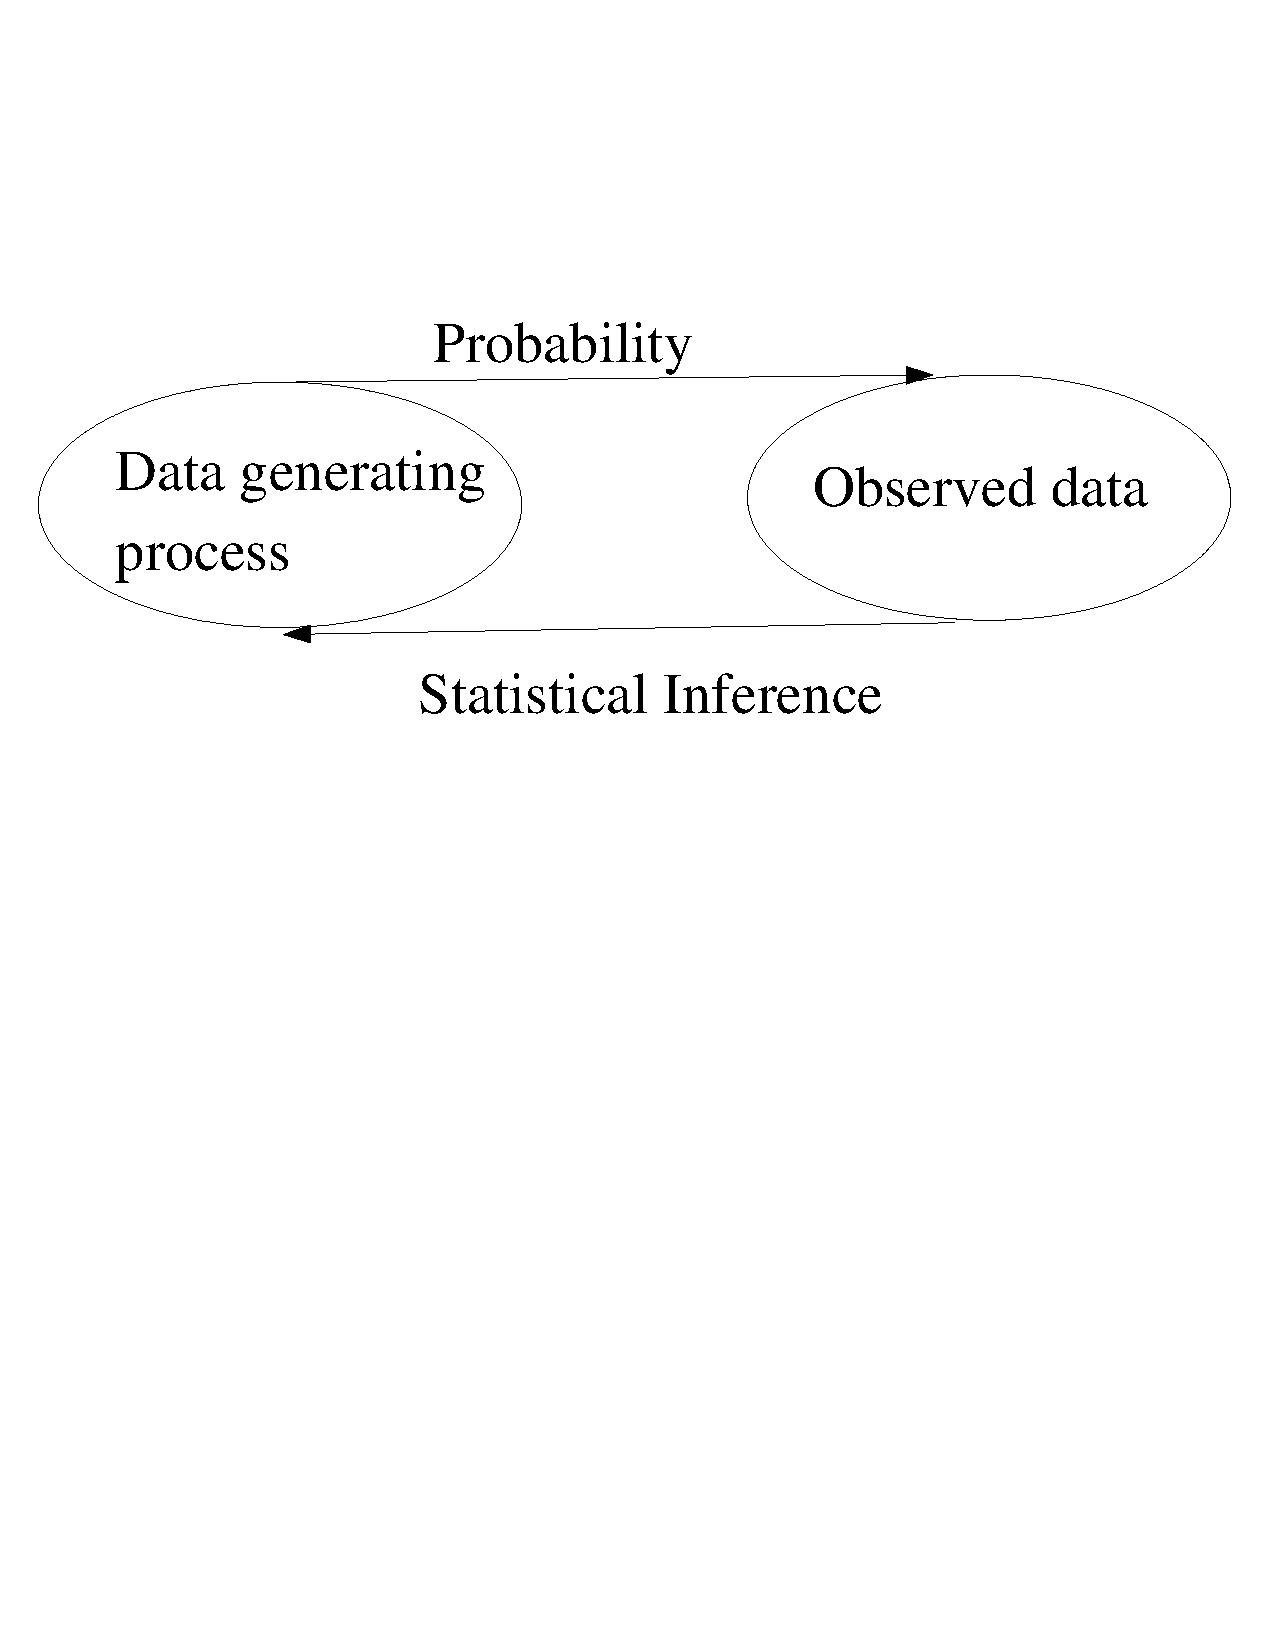
\includegraphics[scale=.4]{probinf3.pdf} % \figonebig{probinf2.pdf}
\end{frame}
%(insert picture from Wasserman, 2005) pg. ix.

\begin{frame}
  \frametitle{Probability}
  {\bf Probability}: Given a data generating process, what are the
  properties of the outcomes (observations)? Simple examples:
\begin{itemize}
\item Example 1: If you know the probability $p$ of ``Heads'' on a coin
  toss is 0.7, and $X$ is the number of heads on 100 independent coin tosses, what is the
  distribution of $X$?
\item Example 2: $(X,Y)$ is bivariate normal with mean 0,
  $(\sigma_1^2,\sigma_2^2)=(1,4)$, covariance=1. What is P$(X>Y^2)$?
\end{itemize}
These are not very complicated calculations. But they are easy to
approximate via simulation/Monte Carlo.
%%Let us write {\tt R} code to do this
%If you have modeled the dynamics of a fluid, how is the fluid likely to behave? How will it behave under different initial conditions?
\end{frame}


\begin{frame}
\frametitle{Why is Computing Important in Probability?}
\begin{itemize}
\item For a complicated statistical model, a probability distribution
  $f$, understanding the properties of the distribution can be
  mathematically challenging
\item However, simulating from $f$ can often be much
  easier. Can use Monte Carlo approximations
\item Goal: Approximate expectation w.r.t. $f$
\item Principle: If we can simulate exactly from $f$ or construct
  (Harris-ergodic) Markov chain with stationary distribution $f$, we
  can approximate this expectation
\item Monte Carlo avoids analytically intractable calculations, numerical
  integration. Convergence rate of estimator is not a function of dimension of
  $f$ (less affected by dimension of the distribution)
%\item Example: ADD INTERESTING SIMPLE EXAMPLE TO SIMULATE FROM
\end{itemize}
\end{frame}

\begin{frame}
  \frametitle{Computing Probabilities via Monte Carlo}
  {\bf Simple idea}: 
\begin{enumerate}
\item Simulate (``pseudo'') random variables from the probability
  model $f(x)$ using computer code, $X_1,X_2,\dots \sim f(x)$
\item Approximate expected value, $\mu=E_f(g(X))$, for 
  real-valued function $g$, compute corresponding sample
  mean, $$\hat{\mu}_m = \frac{\sum_{i=1}^m g(X_i)}{m}$$
\end{enumerate}
Basic probability theory:
\begin{itemize}
\item {\bf Law of large numbers}: sample mean converges to its expectation,
  $\hat{\mu}_m \rightarrow \mu$ as $m\rightarrow \infty$, as long as
  $E_f(g(X)) <\infty$
\item {\bf Central Limit Theorem}: to obtain approximate confidence interval
  for $\mu$ based on $\hat{\mu_m}$
\end{itemize}
\end{frame}

\begin{frame}
  \frametitle{Writing Computer Code for Monte Carlo}
\begin{itemize}
\item Example 1: need command for Binomials, {\tt rbinom}
\item Example 2: simulate bivariate normals, choices:
\begin{itemize}
\item Use {\tt R} package {\tt MASS} and {\tt mvrnorm}
\item (To understand ideas better) Write our own code: (i) enter 
  covariance matrix $\Sigma$, (ii) generate iid
  Norm(0,1) random variates, $\bx$ (iii) compute choleski factor, $C$
  s.t. $CC^T=\Sigma$, and (iv) obtain via multiplication $\bz = C\bx\sim
  N(0,\Sigma)$
\end{itemize}
\item In order to use Monte Carlo, repeat above (procedure for
  generating Binomials or multivariate Normal) many times, then
  calculate sample means
\end{itemize}
\end{frame}

\begin{frame}
  \frametitle{Probability: More Examples}
\begin{itemize}
\item Example 3: Draw values at 30 locations from Gaussian process
  with mean 0 and stationary covariance,
  cov($X_i,X_j$)=$\exp(-d_{ij}/\phi)$, where $d_{ij}$ is Euclidean distance. \\
Call 30-dim r.v., $\bX$. What is $P(X_3 > X_4^2+X_5$)?
\item Example 4: Stochastic model for the spread of an infectious
  disease: Q1. study how disease will spread over space and time for
  different initial conditions/parameter values. Q2. How likely is an
  epidemic?
\item Example 5: Ising model: dependence model for binary data on a
  lattice/undirected graph. Study behavior of system by simulation 
  via Markov chain Monte Carlo (MCMC)
\end{itemize}
\end{frame}

\begin{frame}
\frametitle{Statistical Inference}
{\bf Inference}: Given the outcomes (our observations), what can we
say about the process that generated the data?
\begin{itemize}
\item Example 1 (simple): If you know $X$ (\# of heads on 100 independent
coin tosses) what can you say about $p$?
\begin{itemize}
\item Point estimate for $p$, interval estimate for $p$
\end{itemize}
\item Example 2: Given space-time data on the spread of an infectious 
disease, what are the (unknown) parameters of the stochastic model?
\begin{itemize}
\item Point and interval estimates for parameters
\item Does the model ``fit'' the observations? Idea: simulate from fitted 
model, compare to data. (Back to Monte Carlo)
\end{itemize}
\item Example 3: Observe pairs $(X_1,Y_1),\dots (X_n,
  Y_n)$. Relationship between $X's$ and $Y's$, allowing for
  flexibility (non-linearity + errors)? Predict $Y$ based on $X$?
\end{itemize}
\end{frame}

\begin{frame}
\frametitle{Estimation and Prediction}
{\bf Estimation}: What we say about our fitted model should reflect
our uncertainty (variability) in estimates of the parameter.\\
{\bf Prediction}: We will often use fitted model to make predictions.\\
 Since there is typically randomness in how the data generating 
 process produces the data, our inferences and predictions should 
 account for this variability
\begin{itemize}
\item Sampling distributions, confidence intervals
\item standard errors, bias correction 
\item prediction intervals: variability in predictions from fitted
  model combined with variability from parameter estimates\\ often easy to
  do via simulation-based approach
\end{itemize}
\end{frame}

\begin{frame}
\frametitle{Why is Computing Important in Statistics?}
\begin{itemize}
\item Parameter estimation in a model often involves minimizing/maximizing an objective function
\begin{itemize}
\item Maximum likelihood/penalized maximum likelihood 
\item Nonparametric regression: minimizing an objective function to
  fit a curve to a data set
\end{itemize}
\item Computing standard errors for parameter estimates can be  
  difficult -- asymptotic theory may be hard to derive or inapplicable 
\begin{itemize}
\item Re-sampling methods (bootstrap) for approximating sampling 
  distributions, approximate confidence intervals
\end{itemize}
\item Bayesian inference (alternative to maximum likelihood)
\begin{itemize}
\item Approximating posterior distribution (back to probability) by
  Markov chain Monte Carlo methods
\item Maximizing posterior distribution (back to optimization)
\end{itemize}
\end{itemize}
\end{frame}


\begin{frame}{Advanced Topics/Challenges}
\frametitle{}
\begin{itemize}
\item Likelihood functions are often expensive to evaluate, may
  involve high-dimensional integration
\begin{itemize}
\item Surrogate function methods: minorization-maximization (M-M) algorithms,
  expectation-maximization (E-M) algorithms (special case of MM),
  composite likelihood,...
\item Monte Carlo maximum likelihood, Monte Carlo E-M
\end{itemize}
\item Computational complexity and storage requirements for large
  data, complicated models
\begin{itemize}
\item Divide-and-conquer algorithms for parallelizing
  computing/storage
\item Monte Carlo/MCMC with approximate likelihoods
\end{itemize}
\item New constrained optimization algorithms 
\item + Many research problems in modern probability/statistics
\end{itemize}
\end{frame}

\end{document}